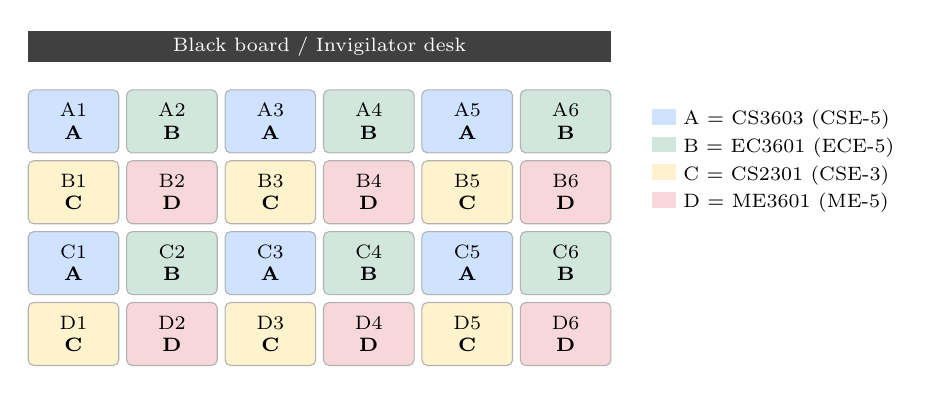
\begin{tikzpicture}[font=\scriptsize]
\definecolor{sA}{RGB}{207,226,255}
\definecolor{sB}{RGB}{209,231,221}
\definecolor{sC}{RGB}{255,243,205}
\definecolor{sD}{RGB}{248,215,218}
\fill[black!75] (0,0.35) rectangle (6*1.25-0.1,0.75);
\node[white] at (3.7,0.55) {Black board / Invigilator desk};
\foreach \s [count=\i from 0] in {A,B,A,B,A,B,C,D,C,D,C,D,A,B,A,B,A,B,C,D,C,D,C,D}{
  \pgfmathtruncatemacro{\r}{int(\i/6)}
  \pgfmathtruncatemacro{\c}{mod(\i,6)}
  \pgfmathtruncatemacro{\cc}{\c+1}
  \fill[s\s,draw=black!30,rounded corners=2pt] (\c*1.25,-\r*0.9) rectangle ++(1.15,-0.8);
  \node[align=center] at (\c*1.25+0.575,-\r*0.9-0.4) {\ifcase\r A\or B\or C\or D\fi\cc\\\textbf{\s}};
}
\node[anchor=west,align=left] at (7.8,-0.9) {
  \tikz\fill[sA](0,0)rectangle(0.3,0.2); A = CS3603 (CSE-5)\\[2pt]
  \tikz\fill[sB](0,0)rectangle(0.3,0.2); B = EC3601 (ECE-5)\\[2pt]
  \tikz\fill[sC](0,0)rectangle(0.3,0.2); C = CS2301 (CSE-3)\\[2pt]
  \tikz\fill[sD](0,0)rectangle(0.3,0.2); D = ME3601 (ME-5)};
\end{tikzpicture}
